\documentclass[11pt,letterpaper]{article}

% ---------------------------------------------------------------- packages
\usepackage[T1]{fontenc}
\usepackage[utf8]{inputenc}
\usepackage{libertinus}
\usepackage[final]{microtype}
\usepackage[margin=1in, headheight=14pt]{geometry}
\usepackage{xcolor}
\usepackage{graphicx}
\usepackage{tikz}
\usetikzlibrary{arrows.meta}
\usepackage{enumitem}
\usepackage{titlesec}
\usepackage{fancyhdr}
\usepackage[font=small, labelfont={sf,bf,color=accent}, labelsep=period, margin=1.5em]{caption}
\usepackage[parfill]{parskip}
\usepackage{hyperref}

% ---------------------------------------------------------------- colours
\definecolor{accent}{HTML}{1D3557}
\definecolor{muted}{HTML}{6B7280}

% ---------------------------------------------------------------- layout
\setlength{\parskip}{0.55em plus 0.15em}

\titleformat{\section}{\sffamily\Large\bfseries\color{accent}}{\thesection}{0.7em}{}
\titlespacing*{\section}{0pt}{2.4ex plus 1ex minus 0.3ex}{1.0ex}

\pagestyle{fancy}
\fancyhf{}
\fancyhead[L]{\sffamily\footnotesize\color{muted} An AI agent harness for scientific experiments}
\fancyhead[R]{\sffamily\footnotesize\color{muted} \thepage}
\renewcommand{\headrulewidth}{0.4pt}
\renewcommand{\headrule}{{\color{muted!40}\hrule height\headrulewidth width\headwidth \vskip-\headrulewidth}}
\fancypagestyle{plain}{\fancyhf{}\renewcommand{\headrulewidth}{0pt}
  \fancyfoot[C]{\sffamily\footnotesize\color{muted}\thepage}}

\hypersetup{
  colorlinks=true, linkcolor=accent, urlcolor=accent, citecolor=accent,
  pdftitle={Building an AI Agent Harness for Conducting Scientific Experiments},
  pdfauthor={Sina Shahandeh},
}
\urlstyle{same}

% Numbered circles for the design decisions
\DeclareRobustCommand{\decnum}[1]{\tikz[baseline=(n.base)]\node[circle, fill=accent, text=white,
  inner sep=0pt, minimum size=1.45em, font=\sffamily\bfseries\footnotesize] (n) {#1};}

\newcommand{\mhapi}{M-HAPI}

% ================================================================ document
\begin{document}
\thispagestyle{plain}

\begin{center}
  {\sffamily\bfseries\LARGE\color{accent}
    Building an AI Agent Harness\\[3pt] for Conducting Scientific Experiments\par}
  \vspace{8pt}
  {\large\itshape Exploring heat-induced aggregation of egg-white proteins\par}
  \vspace{10pt}
  {\sffamily\small Sina Shahandeh \quad\textperiodcentered\quad October 2026\par}
  \vspace{6pt}
  {\color{accent}\rule{0.3\linewidth}{0.8pt}}
\end{center}
\vspace{2pt}

% ----------------------------------------------------------------
\section{Design rationale}

In this short project, I have built a complete end-to-end setup of an AI agent interacting with
the physical world and conducting a scientific experiment. The idea is to convert a 3D printer
into a robotic experimentation platform and have an AI agent autonomously control the movement of
a camera installed on its head and the temperature of its bed
(Figure~\ref{fig:rig}). This setup allows investigation of heat-induced phenomena while the camera
measures color or opacity changes in the materials placed on the bed. Given the temperature range
available on the 3D printer, I decided to investigate the kinetics of aggregation of the protein
molecules present in egg white. Heat-induced changes in protein structure are an important
scientific topic, both in drug design and delivery and in food science.

\begin{figure}[htb]
  \centering
  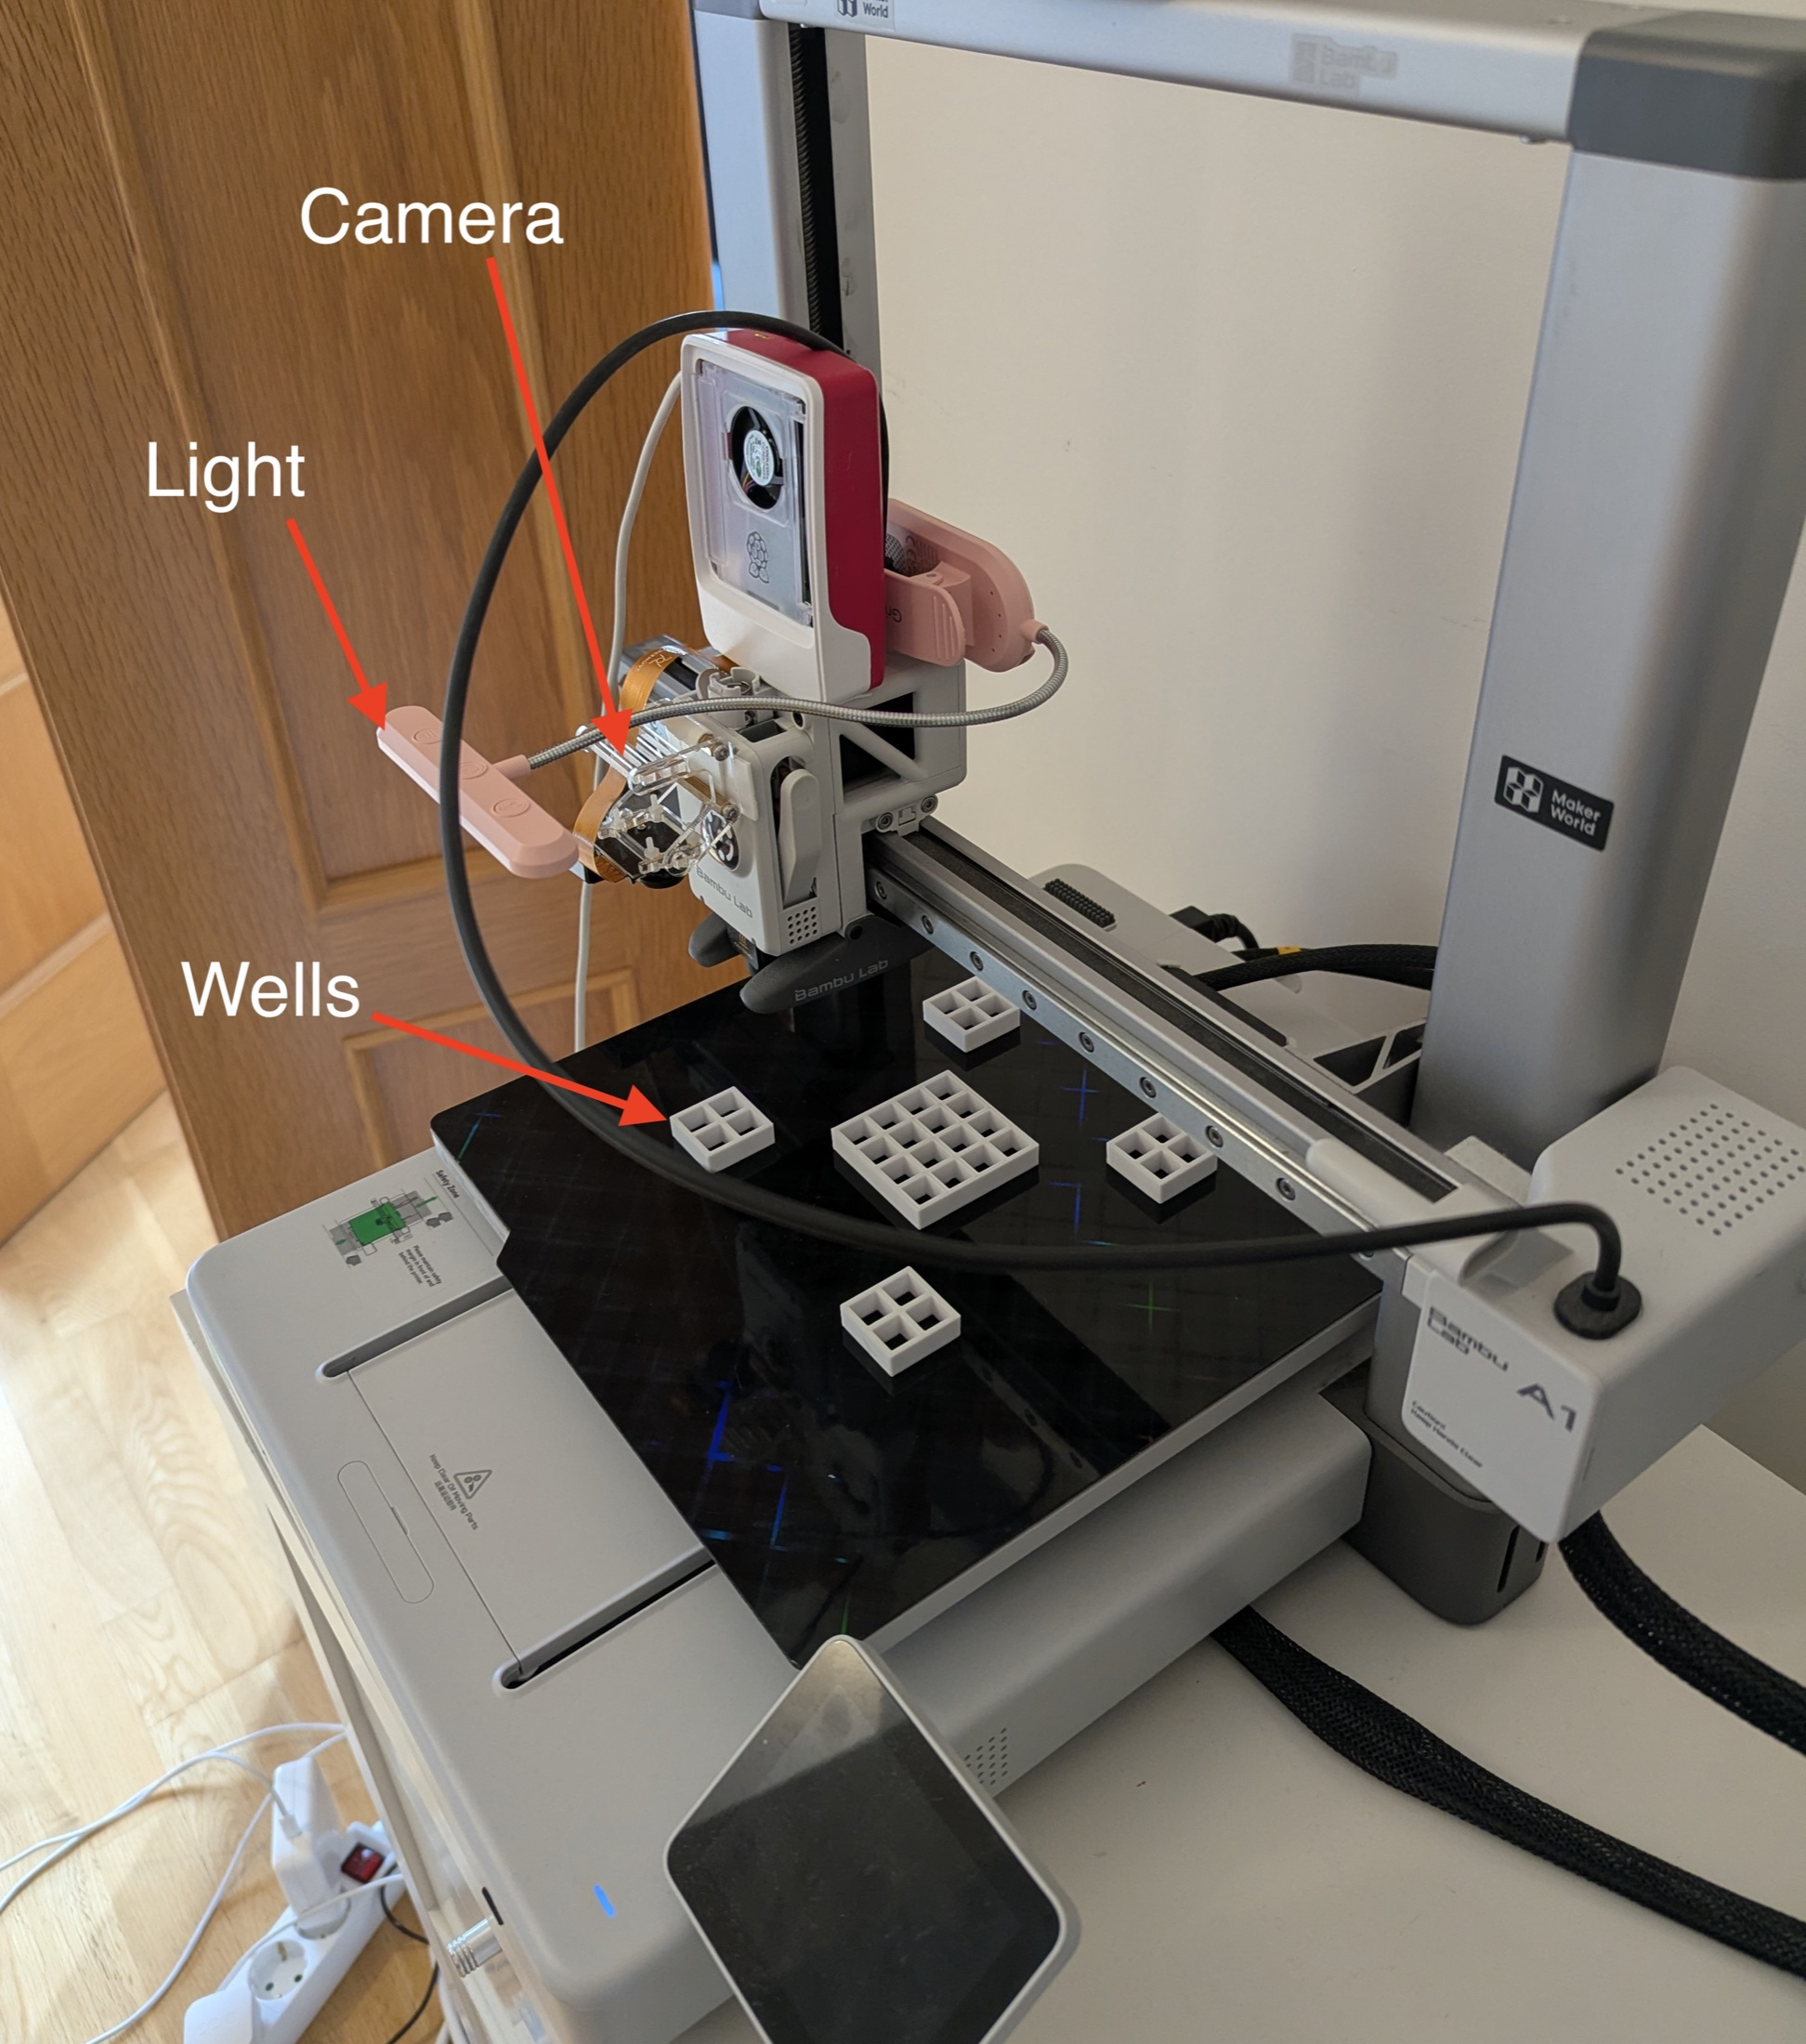
\includegraphics[width=0.56\linewidth]{rig_setup.jpg}
  \caption{The experimental rig. A Bambu Lab A1 3D printer carries a Raspberry Pi camera on its toolhead. A grid of wells is arranged on the heated bed.}
  \label{fig:rig}
\end{figure}

Although current coding agents are able to write scripts to control a 3D printer or a robot, they are not
fundamentally ``in the loop'' during the scientific experiment. Claude Code can write a script to
move a robotic setup, use a camera to take a photo and get feedback from the environment. However,
such a system is fragile; it is hard to implement safety checks coming from the hardware, and it
is hard to scale. Because it is cumbersome for the AI agent to maintain the low-level drivers for robot
control, it limits, through the context window size, how many instruments and how long an experiment
an agent can handle. We need abstractions that separate the actual work of conducting the
scientific experiment from hardware control or higher-level ideation. Conducting scientific experiments has a hierarchical dynamic that is different from tasks such as coding. Figure~\ref{fig:hierarchy} shows this
hierarchy schematically.

\begin{figure}[htb]
  \centering
  % Figure 2: the hierarchy of a scientific experiment, drawn as a sliced pyramid.
% Included by design_rationale.tex with % Figure 2: the hierarchy of a scientific experiment, drawn as a sliced pyramid.
% Included by design_rationale.tex with % Figure 2: the hierarchy of a scientific experiment, drawn as a sliced pyramid.
% Included by design_rationale.tex with \input{fig_hierarchy}.
\definecolor{pyrInk}{HTML}{1D2B45}
\definecolor{pyrTop}{HTML}{1D3557}
\definecolor{pyrBot}{HTML}{BCD3E6}
\definecolor{pyrGround}{HTML}{E8D9AE}
\definecolor{pyrGroundInk}{HTML}{4A3B14}
\definecolor{pyrCmd}{HTML}{D1603D}
\definecolor{pyrObs}{HTML}{23897D}
\begin{tikzpicture}[
    x=1cm, y=1cm,
    cmd/.style={-{Stealth[length=2.8mm,width=2.5mm]}, line width=1.5pt, draw=pyrCmd},
    obs/.style={-{Stealth[length=2.8mm,width=2.5mm]}, line width=1.5pt, draw=pyrObs},
    actor/.style={draw=pyrInk!40, line width=0.6pt, fill=white, rounded corners=8pt,
                  inner xsep=8pt, inner ysep=4pt, font=\sffamily\small\bfseries, text=pyrInk},
    cmdlab/.style={anchor=east, font=\sffamily\footnotesize\itshape, text=pyrCmd},
    obslab/.style={anchor=west, font=\sffamily\footnotesize\itshape, text=pyrObs},
    layer/.style={font=\sffamily\small\bfseries, align=center},
  ]
  \def\a{1.6}   % half-width of the pyramid's top edge
  \def\k{0.46}  % half-width added per cm of depth
  % \slice{top depth}{bottom depth}{fill}{text colour}{label}
  \def\slice#1#2#3#4#5{%
    \pgfmathsetmacro\wt{\a+\k*#1}%
    \pgfmathsetmacro\wb{\a+\k*#2}%
    \fill[#3] (-\wt,-#1) -- (\wt,-#1) -- (\wb,-#2) -- (-\wb,-#2) -- cycle;
    \node[layer, text=#4] at (0,{-(#1+#2)/2}) {#5};}
  % \iface{top depth}{bottom depth}{component}{passed down}{passed up}
  \def\iface#1#2#3#4#5{%
    \pgfmathsetmacro\ax{0.62*(\a+\k*(#1+#2)/2)}%
    \pgfmathsetmacro\ym{-(#1+#2)/2}%
    \draw[cmd] (-\ax,{-#1-0.08}) -- (-\ax,{-#2+0.08});
    \draw[obs] (\ax,{-#2+0.08}) -- (\ax,{-#1-0.08});
    \node[cmdlab] at ({-\ax-0.2},\ym) {#4};
    \node[obslab] at ({\ax+0.2},\ym) {#5};
    \node[actor] at (0,\ym) {#3};}

  % Layers, from the top of the pyramid down
  \slice{0}{0.95}{pyrTop}{white}{Understanding}
  \slice{1.17}{2.12}{pyrTop!80!pyrBot}{white}{Scientific hypothesis}
  \slice{3.37}{4.32}{pyrTop!60!pyrBot}{white}{Experiment protocol design}
  \slice{5.57}{6.52}{pyrTop!38!pyrBot}{white}{Collection of experimental sub-tasks}
  \slice{7.77}{8.92}{pyrTop!14!pyrBot}{pyrInk}{Robot hardware control\\[-1pt]
    {\footnotesize\mdseries to run each individual task}}
  \slice{10.17}{11.12}{pyrGround}{pyrGroundInk}{The physical system under study}

  % Interfaces between neighboring layers
  \pgfmathsetmacro\ax{0.62*(\a+\k*(2.12+3.37)/2)}
  \draw[cmd] (-\ax,-2.20) -- (-\ax,-3.29);
  \draw[obs] (\ax,-3.29) -- (\ax,-2.20);
  \node[cmdlab] at ({-\ax-0.2},-2.745) {abstract tasks};
  \node[obslab] at ({\ax+0.2},-2.745) {observations};
  \iface{4.32}{5.57}{Experimental Agent}{tasks}{experimental results}
  \iface{6.52}{7.77}{Model--Hardware API (M-HAPI)}{abstract actions}{science metrics}
  \iface{8.92}{10.17}{Firmware}{actuation}{environment sensing}

  % Legend
  \begin{scope}[shift={(0,-11.85)}]
    \draw[cmd] (-4.9,0.2) -- (-4.9,-0.2);
    \node[anchor=west, font=\sffamily\footnotesize, text=pyrInk] at (-4.7,0)
      {passed down to the layer below};
    \draw[obs] (0.7,-0.2) -- (0.7,0.2);
    \node[anchor=west, font=\sffamily\footnotesize, text=pyrInk] at (0.9,0)
      {passed up to the layer above};
  \end{scope}
\end{tikzpicture}
.
\definecolor{pyrInk}{HTML}{1D2B45}
\definecolor{pyrTop}{HTML}{1D3557}
\definecolor{pyrBot}{HTML}{BCD3E6}
\definecolor{pyrGround}{HTML}{E8D9AE}
\definecolor{pyrGroundInk}{HTML}{4A3B14}
\definecolor{pyrCmd}{HTML}{D1603D}
\definecolor{pyrObs}{HTML}{23897D}
\begin{tikzpicture}[
    x=1cm, y=1cm,
    cmd/.style={-{Stealth[length=2.8mm,width=2.5mm]}, line width=1.5pt, draw=pyrCmd},
    obs/.style={-{Stealth[length=2.8mm,width=2.5mm]}, line width=1.5pt, draw=pyrObs},
    actor/.style={draw=pyrInk!40, line width=0.6pt, fill=white, rounded corners=8pt,
                  inner xsep=8pt, inner ysep=4pt, font=\sffamily\small\bfseries, text=pyrInk},
    cmdlab/.style={anchor=east, font=\sffamily\footnotesize\itshape, text=pyrCmd},
    obslab/.style={anchor=west, font=\sffamily\footnotesize\itshape, text=pyrObs},
    layer/.style={font=\sffamily\small\bfseries, align=center},
  ]
  \def\a{1.6}   % half-width of the pyramid's top edge
  \def\k{0.46}  % half-width added per cm of depth
  % \slice{top depth}{bottom depth}{fill}{text colour}{label}
  \def\slice#1#2#3#4#5{%
    \pgfmathsetmacro\wt{\a+\k*#1}%
    \pgfmathsetmacro\wb{\a+\k*#2}%
    \fill[#3] (-\wt,-#1) -- (\wt,-#1) -- (\wb,-#2) -- (-\wb,-#2) -- cycle;
    \node[layer, text=#4] at (0,{-(#1+#2)/2}) {#5};}
  % \iface{top depth}{bottom depth}{component}{passed down}{passed up}
  \def\iface#1#2#3#4#5{%
    \pgfmathsetmacro\ax{0.62*(\a+\k*(#1+#2)/2)}%
    \pgfmathsetmacro\ym{-(#1+#2)/2}%
    \draw[cmd] (-\ax,{-#1-0.08}) -- (-\ax,{-#2+0.08});
    \draw[obs] (\ax,{-#2+0.08}) -- (\ax,{-#1-0.08});
    \node[cmdlab] at ({-\ax-0.2},\ym) {#4};
    \node[obslab] at ({\ax+0.2},\ym) {#5};
    \node[actor] at (0,\ym) {#3};}

  % Layers, from the top of the pyramid down
  \slice{0}{0.95}{pyrTop}{white}{Understanding}
  \slice{1.17}{2.12}{pyrTop!80!pyrBot}{white}{Scientific hypothesis}
  \slice{3.37}{4.32}{pyrTop!60!pyrBot}{white}{Experiment protocol design}
  \slice{5.57}{6.52}{pyrTop!38!pyrBot}{white}{Collection of experimental sub-tasks}
  \slice{7.77}{8.92}{pyrTop!14!pyrBot}{pyrInk}{Robot hardware control\\[-1pt]
    {\footnotesize\mdseries to run each individual task}}
  \slice{10.17}{11.12}{pyrGround}{pyrGroundInk}{The physical system under study}

  % Interfaces between neighboring layers
  \pgfmathsetmacro\ax{0.62*(\a+\k*(2.12+3.37)/2)}
  \draw[cmd] (-\ax,-2.20) -- (-\ax,-3.29);
  \draw[obs] (\ax,-3.29) -- (\ax,-2.20);
  \node[cmdlab] at ({-\ax-0.2},-2.745) {abstract tasks};
  \node[obslab] at ({\ax+0.2},-2.745) {observations};
  \iface{4.32}{5.57}{Experimental Agent}{tasks}{experimental results}
  \iface{6.52}{7.77}{Model--Hardware API (M-HAPI)}{abstract actions}{science metrics}
  \iface{8.92}{10.17}{Firmware}{actuation}{environment sensing}

  % Legend
  \begin{scope}[shift={(0,-11.85)}]
    \draw[cmd] (-4.9,0.2) -- (-4.9,-0.2);
    \node[anchor=west, font=\sffamily\footnotesize, text=pyrInk] at (-4.7,0)
      {passed down to the layer below};
    \draw[obs] (0.7,-0.2) -- (0.7,0.2);
    \node[anchor=west, font=\sffamily\footnotesize, text=pyrInk] at (0.9,0)
      {passed up to the layer above};
  \end{scope}
\end{tikzpicture}
.
\definecolor{pyrInk}{HTML}{1D2B45}
\definecolor{pyrTop}{HTML}{1D3557}
\definecolor{pyrBot}{HTML}{BCD3E6}
\definecolor{pyrGround}{HTML}{E8D9AE}
\definecolor{pyrGroundInk}{HTML}{4A3B14}
\definecolor{pyrCmd}{HTML}{D1603D}
\definecolor{pyrObs}{HTML}{23897D}
\begin{tikzpicture}[
    x=1cm, y=1cm,
    cmd/.style={-{Stealth[length=2.8mm,width=2.5mm]}, line width=1.5pt, draw=pyrCmd},
    obs/.style={-{Stealth[length=2.8mm,width=2.5mm]}, line width=1.5pt, draw=pyrObs},
    actor/.style={draw=pyrInk!40, line width=0.6pt, fill=white, rounded corners=8pt,
                  inner xsep=8pt, inner ysep=4pt, font=\sffamily\small\bfseries, text=pyrInk},
    cmdlab/.style={anchor=east, font=\sffamily\footnotesize\itshape, text=pyrCmd},
    obslab/.style={anchor=west, font=\sffamily\footnotesize\itshape, text=pyrObs},
    layer/.style={font=\sffamily\small\bfseries, align=center},
  ]
  \def\a{1.6}   % half-width of the pyramid's top edge
  \def\k{0.46}  % half-width added per cm of depth
  % \slice{top depth}{bottom depth}{fill}{text colour}{label}
  \def\slice#1#2#3#4#5{%
    \pgfmathsetmacro\wt{\a+\k*#1}%
    \pgfmathsetmacro\wb{\a+\k*#2}%
    \fill[#3] (-\wt,-#1) -- (\wt,-#1) -- (\wb,-#2) -- (-\wb,-#2) -- cycle;
    \node[layer, text=#4] at (0,{-(#1+#2)/2}) {#5};}
  % \iface{top depth}{bottom depth}{component}{passed down}{passed up}
  \def\iface#1#2#3#4#5{%
    \pgfmathsetmacro\ax{0.62*(\a+\k*(#1+#2)/2)}%
    \pgfmathsetmacro\ym{-(#1+#2)/2}%
    \draw[cmd] (-\ax,{-#1-0.08}) -- (-\ax,{-#2+0.08});
    \draw[obs] (\ax,{-#2+0.08}) -- (\ax,{-#1-0.08});
    \node[cmdlab] at ({-\ax-0.2},\ym) {#4};
    \node[obslab] at ({\ax+0.2},\ym) {#5};
    \node[actor] at (0,\ym) {#3};}

  % Layers, from the top of the pyramid down
  \slice{0}{0.95}{pyrTop}{white}{Understanding}
  \slice{1.17}{2.12}{pyrTop!80!pyrBot}{white}{Scientific hypothesis}
  \slice{3.37}{4.32}{pyrTop!60!pyrBot}{white}{Experiment protocol design}
  \slice{5.57}{6.52}{pyrTop!38!pyrBot}{white}{Collection of experimental sub-tasks}
  \slice{7.77}{8.92}{pyrTop!14!pyrBot}{pyrInk}{Robot hardware control\\[-1pt]
    {\footnotesize\mdseries to run each individual task}}
  \slice{10.17}{11.12}{pyrGround}{pyrGroundInk}{The physical system under study}

  % Interfaces between neighboring layers
  \pgfmathsetmacro\ax{0.62*(\a+\k*(2.12+3.37)/2)}
  \draw[cmd] (-\ax,-2.20) -- (-\ax,-3.29);
  \draw[obs] (\ax,-3.29) -- (\ax,-2.20);
  \node[cmdlab] at ({-\ax-0.2},-2.745) {abstract tasks};
  \node[obslab] at ({\ax+0.2},-2.745) {observations};
  \iface{4.32}{5.57}{Experimental Agent}{tasks}{experimental results}
  \iface{6.52}{7.77}{Model--Hardware API (M-HAPI)}{abstract actions}{science metrics}
  \iface{8.92}{10.17}{Firmware}{actuation}{environment sensing}

  % Legend
  \begin{scope}[shift={(0,-11.85)}]
    \draw[cmd] (-4.9,0.2) -- (-4.9,-0.2);
    \node[anchor=west, font=\sffamily\footnotesize, text=pyrInk] at (-4.7,0)
      {passed down to the layer below};
    \draw[obs] (0.7,-0.2) -- (0.7,0.2);
    \node[anchor=west, font=\sffamily\footnotesize, text=pyrInk] at (0.9,0)
      {passed up to the layer above};
  \end{scope}
\end{tikzpicture}

  \caption{The hierarchy of a scientific experiment, from the physical system under study up to
    understanding. Each arrow shows what one layer passes to the next level; the boxes name the
    component that works at each interface in this project.}
  \label{fig:hierarchy}
\end{figure}

An agent performing at any of the levels needs specific information about the layers above and
below it, but not all of it. Orchestration of activities across the layers is also important.
The following are my design decisions for building this robotic experimentation system:

\begin{enumerate}[label={\decnum{\arabic*}}, leftmargin=2.3em, labelsep=0.6em, itemsep=0.5em,
  topsep=0.3em]
  \item \textbf{Build a custom AI agent harness as a Python backend.} It holds the context about
    the system setup and tools as the system prompt, and the experiment protocol as the first user
    prompt. The harness calls the model API to decide which tools to call and how to present
    experiment results.

  \item \textbf{Build a Model--Hardware API (\mhapi) protocol:} an interface between the robotic
    control and the experiment sub-tasks. The need for this abstraction is quite clear, given that
    the robotic hardware interacts with the world through its own firmware and exposes only basic,
    fundamental action blocks (move the nozzle to an $x, y, z$ position). This is too low-level
    for the experimental sub-tasks. The recently announced Model Hardware Standard (not yet
    released at the time of writing) aims at the same problem. For my Model--Hardware API, I
    prompted Claude Code to explore the documentation for the Bambu Lab 3D printer and for the
    camera connected to a Raspberry Pi, and to set up basic primitives such as
    \texttt{set\_temperature()} or \texttt{get\_well\_opacity\_measurement(well\_label)}. Writing
    the spec documentation and exploring and fixing hardware issues took a significant amount of
    the time for this project. A reliable and well-designed Model--Hardware interface is crucial.

  \item \textbf{Build a digital twin of the system} to test the harness and the \mhapi{} together
    before running physical experiments. A well-designed and well-scoped digital twin can uncover
    mistakes and shortcomings before the hardware is used. This simulated environment interfaces
    with the same \mhapi{} and tries to mimic as much physics as possible in the core simulation
    engine. You can see it working as an experiment dashboard at
    \url{https://34-9-34-15.sslip.io/}. This web app interfaces with the agent harness running in
    the background as well as with the simulation engine, and twins the entire system end to end.
\end{enumerate}

In the video you will see the same dashboard connected to the robot hardware, showing the actual
camera feeds and the experimental data coming from the rig.

% ----------------------------------------------------------------
\section{Significance of this project and further work}

What I showed here is a simple yet complete example of an end-to-end system running an AI agent
on an experimentation platform and putting an LLM in the loop with the physical system. The
significance of this work is this very abstraction, and how we put the LLM in the loop. Let me
explain with a contrasting example. As I was experimenting with the \mhapi, I asked Claude Code to
control the setup directly and obtain the kinetic coefficient of protein aggregation (the rate of
egg-white whitening). Claude Code wrote a script to run this experiment loop, and the robot
executed it with no issues. I later realized the egg white had not completely filled the well, so
the opacity measurements would be off. This mistake would not have been discovered had I not
looked at the wells manually. This is because the LLM's reasoning was not inside the loop for
every frame. Claude did not look at every well as it was conducting the experiment; with the wrong
abstraction, it outsourced the loop to an automated script. This is the same pattern used in a
coding environment, and the model is post-trained for it very well. But the coding environment
does not have the variability that exists in the physical world.

In contrast, while I was conducting the same experiment with the custom harness, the agent asked
me to fill four wells, and I forgot to fill two. Because the LLM had to take a
photo of each well and get the opacity number through an \mhapi{} tool call, rather than write
code, the model was induced to reason about each image and to stay constantly inside the
experimental observations, at the obvious cost of more test-time compute. In this run, the agent notified me there was something wrong with the two wells, and I had to instruct it to ignore and run the experiment with $n=2$.

This brings us to the first immediate direction for further work: what is the optimal level of
abstraction across the six levels of the pyramid in Figure~\ref{fig:hierarchy}? I am actually not
satisfied with the current, hard-coded version of the \mhapi. Reading the press release for Anthropic's Model Hardware Standard, it appears that an AI agent interviews the scientist on how to set things up, but this is a
one-time process. A better version would be an adaptive system that adjusts the boundary between
agentic, LLM-reasoned work and hard-coded abstraction. Or I can imagine the Model--Hardware
interface itself being run dynamically by a faster, cheaper LLM rather than by code, where the LLM
produces code on the fly or uses some sort of domain-specific language to execute hardware
commands. This would allow the harness to adapt to the complexity and noise of the physical
system, and the trajectories of experimentation could be used directly to post-train the LLM for
scientific tasks. Learning from the Bitter Lesson, one should try to avoid hand-crafting
abstractions between the levels, and instead let the model dynamically pay attention to the high-
and low-level components of the experimental loop, using sub-agent processes. That is how a
scientist moves between understanding at the high level and kneeling down at the instruments to
fix the apparatus.

Another direction for further work is to incorporate safety mechanisms in the experimental loop. Currently, certain safety measures are included in the \mhapi; for example, the bed temperature cannot
be set above 100\,\textdegree C. But thinking through every safety issue and hard-coding it into
the API layers is neither the most flexible nor the most robust approach. I can imagine a
separate, always-on agentic loop running across the abstraction layers and monitoring for various
safety issues, guided by a broad system prompt rather than one that specifies rigid details. I
wrote the spec for this but have not had time to implement and test it.

% ----------------------------------------------------------------
\section{Time spent and logistics}

The most time-consuming part of this project was building the physical setup: I had to retrofit
the 3D printer, glue a camera to the filament nozzle, and test and calibrate the light and fixtures
to be able to measure the opacity of egg white inside each well. The coding task itself was mostly
writing the spec documents for the Model--Hardware API and the harness (3~hours). Once the spec and
the setup were clean and accurate, Claude one-shotted most of the code. Testing took another
1--2~hours, and writing this document another 1.5~hours. I have yet to edit the video I took during
the experiment, which should take about 30~minutes.

% ----------------------------------------------------------------
\section{Final words}

This was a very fun project. I am a theoretical and computational scientist, but I love working
and dealing with physical labs and instruments. This project brought me back to the time I was a
teenager doing DIY projects, something I have picked up again now, playing with my kids.

It was beautiful and magical to see Claude controlling the printer, looking through the camera and
reasoning. In one session it saw me in the printer's side camera and recognized that it must be
me! We are at the onset of another Claude Code moment, but for complete scientific
exploration.

As we develop more capable models and harnesses for science, safety issues across the lab and
model execution, as well as the broader use of AI tools for science at a high level, become even
more important. We should take on these concerns at the same time as the tooling and the
post-training of the model are being developed, rather than as an afterthought at deployment time.

\end{document}
